\chapter{Liveness \Author{B. Boissinot \andAuthor F. Rastello}}
\label{chapter:ssa_tells_nothing_of_liveness}
\inputpath{part3}{ssa_tells_nothing_of_liveness}
\inputprogress
\newcommand{\name}[1]{#1}
\newcommand{\firm}{\name{LibFirm}}
\newcommand{\lao}{\name{LAO}}
\newcommand{\stm}{\name{STMicroelectronics}}
\newcommand{\Nat}{\mathbb{N}}
\newcommand{\void}[1]{ }
\newcommand{\lstart}{\textsf{start}}
\newcommand{\paper}{paper\xspace}
\newcommand{\vundef}{\Box}
\newcommand{\domzone}[1]{\mathit{dom}({#1})}
\newcommand{\sdomzone}[1]{\mathit{sdom}({#1})}
\newcommand{\prenum}[1]{\mathit{prenum}({#1})}
\newcommand{\back}[1]{\mathcal{B}_{#1}}
\newcommand{\lb}[1]{\mathbf{#1}}
\newcommand{\ldef}[1]{\mathit{def}(\var{#1})}
\newcommand{\luse}[1]{\mathit{uses}(\var{#1})}
\newcommand{\reach}[2]{{#1}\rightarrow {#2}}
\newcommand{\redreach}[2]{{#1}\rightharpoondown {#2}}
\newcommand{\red}[1]{\widetilde{#1}}
\newcommand{\BEsrc}{V^\otimes}
\newcommand{\BEtgt}{V^\odot}
\newcommand{\BE}{E^\uparrow}
\newcommand{\Tqa}{T_{(q,\var a)}}
\newcommand{\alain}[1]{{\color{red} #1}}
\newcommand{\reduced}{forward}
\newcommand{\Reduced}{Forward}
\def\Live{\textrm{Live}}
\def\LiveOut{\textrm{LiveOut}}
\def\LiveIn{\textrm{LiveIn}}
\def\PhiKill{\textrm{PhiDefs}}
\def\PhiUses{\textrm{PhiUses}}
\def\Kill{\textrm{Defs}}
\def\Exit{\textrm{Exit}}
\def\Entry{\textrm{Entry}}
\def\UpExp{\textrm{UpwardExposed}}
\def\cfgsuccs{\textrm{CFG\_succs}}
\def\union{\cup}
\def\Def{\textrm{def}}
\def\phidefedge{\texttt{phidef\_edge}}
\def\phiuseedge{\texttt{phiuse\_edge}}
\def\top{\textrm{top}}
\def\push{\textrm{push}}
\def\pop{\textrm{pop}}
\newcommand{\Func}[2]{\textsf{{\bf Function} #1}\\\Begin{#2}}
\newcommand{\reducedGraph}{forward control-flow graph}
\newcommand{\Comment}{C}

\section{Introduction}
This chapter illustrates the use of strict SSA properties to simplify and accelerate \emph{liveness analysis}, \ie an analysis that determines for all variables the set of program points where the variables' values are potentially used by subsequent operations.
Liveness information is essential to solve storage assignment problems, eliminate redundancies, and perform code motion.
For instance, optimizations like software pipelining, trace scheduling, register-sensitive redundancy elimination, if-conversion, as well as register allocation heavily rely on liveness information.

% What is the problem

Traditionally, liveness information is obtained by data-flow analysis:
liveness sets are computed for all basic blocks and variables simultaneously by solving a set of data-flow equations.
These equations are usually solved by an iterative algorithm, propagating information backwards through the control-flow graph (CFG) until a fixed point is reached and the liveness sets stabilize.
The number of iterations depends on the control-flow structure of the considered program, more precisely on the structure of its loops (see discussions in Section~\ref{sec:liveness:further}).

% What is our main result. I think this is simple enough so that is can be put it in the introduction
In this chapter, we show that, for strict SSA-form programs, the live-range of a variable, say~$v$, has nice properties that can be expressed in terms of loop nesting forest of the CFG and its corresponding directed acyclic graph, the forward-CFG\index{forward control-flow graph}.
Informally speaking, and restricted to reducible CFGs, those properties are:
\begin{itemize}
\item
	$v$ is live at a program point~$q$ if and only if $v$ is live at the entry~$h$ of the largest loop/basic-block (highest node in the loop nesting forest\index{loop nesting forest}) that contains~$q$ but not the definition of~$v$.
\item
	$v$ is live at~$h$ if and only if there is a path in the forward-CFG from~$h$ to a use of~$v$ that does not contain the definition.
\end{itemize}

% What is our solution for liveness sets computation

A direct consequence of this property is the possible design of a data-flow algorithm that computes liveness sets \emph{without the requirement of any iteration} to reach a fixed point:
at most two passes over the CFG are necessary.
The first pass, very similar to traditional data-flow analysis, computes partial liveness sets by traversing the forward-CFG backwards.
The second pass refines the partial liveness sets and computes the final solution by propagating forward along the loop-nesting forest.
For the sake of clarity, we first present the algorithm for reducible CFGs.
Irreducible CFGs can be handled with a slight variation of the algorithm, with no need to modify the CFG itself (Section~\ref{sec:irreducible}).

% Other var-by-var etc approaches for liveness sets computation
Another approach to liveness analysis more closely follows the classical definition of liveness:
a variable is live at a program point~$q$, if~$q$ belongs to a path of the CFG leading from a definition of that variable to one of its uses without passing through another definition of the same variable.
Therefore, the live-range of a variable can be computed using a backward traversal starting on its uses and stopping when reaching its (unique) definition.

% Our liveness check solution
Another application of the properties of live-ranges under strict SSA-form is the design of an extremely simple liveness check algorithm.
In contrast to classical data-flow analyses, liveness check does not provide the set of variables live at a block, but its characteristic function.
Liveness check provides a query system to answer questions such as ``Is variable~$v$ live at location~$q$?''.
Its main features are:
\begin{compactenum}
\item
	The algorithm itself consists of two parts, a \emph{precomputation} part, and an \emph{online} part executed at each liveness query.
	It is not based on setting up and subsequently solving data-flow equations.
\item
	The precomputation is \emph{independent of variables,} it only depends on the structure of the control-flow graph.
	Hence, precomputed information \emph{remains valid} upon adding or removing variables or their uses.
\item
	An actual query uses the def-use chain (see below) of the variable in question and determines the answer essentially by testing membership in precomputed sets.
\end{compactenum}

% Layout
In the next section we repeat basic definitions relevant in our context and provide the theoretical foundations.
Thereafter we present algorithms to compute liveness sets:
The two-pass data-flow algorithm in Section~\ref{sec:data-flow} and the algorithms based on path-exploration in Section~\ref{sec:path-explore}.
In Section~\ref{sec:live-check}, we present the liveness checking algorithm.


\section{Definitions}
Liveness is a property relating program points to sets of variables which are considered to be \emph{live} at these program points.
Intuitively, a variable is considered live at a given program point when its value is used in the future by any dynamic execution.
Statically, liveness can be approximated by following paths, backwards, through the control-flow graph leading from uses of a given variable to its definitions - or in the case of SSA form to its unique definition.
The variable is live at all program points along these paths.
For a CFG node~$q$, representing an instruction or a basic block, a variable $\var{v}$ is \emph{live-in} at~$q$ if there is a path, not containing the definition of $\var{v}$, from~$q$ to a node where $\var{v}$ is used.
It is \emph{live-out} at~$q$ if it is live-in at some successor of~$q$.

The computation of live-in and live-out sets at the entry and the exit of basic blocks is usually termed \emph{liveness analysis}.
It is indeed sufficient to consider only these sets at basic-block boundaries since liveness within a basic block is trivial to recompute from its live-out set.
\emph{Live-ranges} are closely related to liveness.
Instead of associating program points with sets of live variables, the live-range of a variable specifies the set of program points where that variable is live.
Live-ranges in programs under strict SSA form exhibit certain useful properties (see Chapter~, some of which have been exploited for register allocation~\cite{HGG:2006:RA_SSA,bouchez:lcpc}, some of which can be exploited during the computation of liveness information.
The special behavior of $\phi$-functions often causes confusion on where exactly its operands are actually used and defined.

For a regular operation, variables are used and defined where the operation takes place.
However, the semantics of \phifuns\ (and in particular the actual place of \phiuses) should be defined carefully, especially when dealing with SSA destruction.
In all algorithms for SSA destruction, such as~\cite{briggs98practical,sreedhar:ssa,boissinot:2009:ssadestruction}, a use in a \phifun is considered live somewhere inside the corresponding predecessor block, but, depending on the algorithm and, in particular, the way copies are inserted, it may or may not be considered as live-out for that predecessor block.
Similarly, the definition of a \phifun is always considered to be at the beginning of the block, but, depending on the algorithm, it may or may not be marked as live-in for the block.
%These subtleties need to be taken into account when building liveness sets.
To make the description of algorithms easier, we follow the definition by Sreedhar~\cite{sreedhar:ssa}.
For a $\phi$-function $a_0 = \phi(a_1, \ldots, a_n)$ in block~$B_0$, where $a_i$ comes from block~$B_i$
\begin{compactitem}
\item
	$a_0$ is considered to be live-in for $B_0$, but, with respect to this $\phi$-function, it is not live-out for $B_i$, $i>0$.
\item
	$a_i$, $i>0$, is considered to be live-out of $B_i$, but, with respect to this $\phi$-function, it is not live-in for $B_0$.
\end{compactitem}
\todo[``with respect to this phi-functions'' means ``if no other cause for live-in/out exists''?]
% This way, each use of a \phifun is considered as live-out of the corresponding predecessor block (but not live-in of the block where the variable defined by the \phifun is considered to be live-in for the block where it is defined.
This corresponds to placing a copy of $a_i$ to $a_0$ on each edge from $B_i$ to $B_0$.
The data-flow equations given hereafter and the presented algorithms follow the same semantics.
They require minor modifications when other $\phi$-semantics are desired.
We will come back to these subtleties in Section~\ref{sec:correctnessdebase}.

\section{Data-Flow Approaches}
\label{sec:data-flow}

A well-known and frequently used approach to compute the live-in and live-out sets of basic blocks is backward data-flow analysis~\cite{appel:2002:modern}.
The liveness sets are given by a set of \emph{equations} that relate the \emph{upward-exposed uses} and the \emph{definitions} occurring within a basic block to the live-in and live-out sets of the predecessors and successors in the \@CFG.
A use is said to be \emph{upward-exposed} when a variable is used within a basic block and no definition of the same variable precedes the use locally within that basic block.
The sets of upward-exposed uses and definitions do not change during liveness analysis and can thus be precomputed.

In the following equations, we denote by $\PhiKill(B)$ the variables defined by \phifuns at entry of the block~$B$ and by $\PhiUses(B)$ the set of variables used in a \phifun at entry of a block successor of the block~$B$.

\begin{eqnarray*}
	\LiveIn(B) & = & \PhiKill(B) \cup \UpExp(B) \cup \,(\LiveOut(B)\setminus \Kill(B)) \\
	\LiveOut(B)& = &
	\textstyle \bigcup_{S \in \textrm{succs}(B)} (\LiveIn(S) \setminus
	\PhiKill(S)) \cup\, \PhiUses(B)
\end{eqnarray*}

\subsection{Liveness Sets On Reducible Graphs}
\label{sec:forreducible}

Instead of computing a fixed point, we show that liveness information can be derived in two passes over the control-flow graph.
The first version of the algorithm requires the CFG to be reducible.
We then show that arbitrary control-flow graphs can be handled elegantly and with no additional cost, except for a cheap pre-processing step on the loop-nesting forest.

The key properties of live-ranges under strict SSA form that we exploit for this purpose and that we will formalize and prove later on, can be outlined as follow:
\begin{enumerate}
\item
	Let~$q$ be a CFG node that does not contain the definition~$d$ of a variable~$v$, $h$ be the header of the maximal loop containing~$q$ but not~$d$.
	Let~$h$ be~$q$ if such maximal loop does not exist.
	Then~$v$ is live-in at~$q$ if and only if there exists a forward path from~$h$ to a use of~$v$ without going through the definition of~$v$.
\item
	If~$v$ is live-in at the header of a loop then it is live at all nodes inside the loop.
\end{enumerate}
Those two properties pave the way for describing the two steps that make up our liveness set algorithm:
\begin{compactenum}
\item
	A backward pass propagates partial liveness information upwards using a post-order traversal of the \@CFG.
\item
	The partial liveness sets are then refined by traversing the loop-nesting forest, propagating liveness from loop-headers down to all basic blocks within loops.
\end{compactenum}
Algorithm~\ref{alg:twopass} shows the necessary initialization and the high-level structure to compute liveness in two passes.

\begin{algorithm}[H]
    \Func{Compute\_LiveSets\_SSA\_Reducible(CFG)}{
      \For{each basic block~$B$}{
          mark~$B$ as unprocessed\;
      }
      \textsf{DAG\_DFS}($R$) \Comment~$R$ is the CFG root node\;
      \For{each root node~$L$ of the loop-nesting forest}{
        \textsf{LoopTree\_DFS}($L$)
      }
    }
    \caption{Two-pass liveness analysis: reducible \@CFG.}
  \label{alg:twopass}
\end{algorithm}

The post-order traversal is shown in Algorithm~\ref{alg:dag_dfs}, which performs a simple depth-first search and associates every basic block of the CFG with partial liveness sets.
The algorithm roughly corresponds to the precomputation step of the traditional iterative data-flow analysis.
However, loop-edges are not considered during the traversal (Line~\ref{alg:dag_dfs:loop_edge}).
Recalling the definition of liveness for \phifuns, $\PhiUses(B)$ denotes the set of variables live-out of basic block~$B$ due to uses by \phifuns in~$B$'s successors.
Similarly, $\PhiKill(B)$ denotes the set of variables defined by a \phifun in~$B$.

\begin{algorithm}[H]
    \Func{DAG\_DFS(block~$B$)}{
      \For{each $S\in\textrm{succs}(B)$ if $(B,S)$ is not a loop-edge}{\label{alg:dag_dfs:loop_edge}
        \lIf{$S$ is unprocessed}{\textsf{DAG\_DFS}($S$)}\label{alg:dag_dfs:irreducible_dfs}
      }
      $Live=\PhiUses(B)$ \label{alg:dag_dfs:phi_use}
      \For{each $S\in\textrm{succs}(B)$ if $(B,S)$ is not a loop-edge}{
        $Live = Live \union (\LiveIn(S) \setminus \PhiKill(S))$ \label{alg:dag_dfs:phi_kill_minus}\label{alg:dag_dfs:irreducible}\;
      }
      $\LiveOut(B)=Live$\;
      \For{each program point~$p$ in~$B$, backward}{
        remove variables defined at~$p$ from $Live$\;
        add uses at~$p$ to $Live$\;
      }
      $\LiveIn(B)=Live \union \PhiKill(B)$ \label{alg:dag_dfs:phi_kill_union}\;
      mark~$B$ as processed\;
    }
  \caption{Partial liveness, with post-order traversal.}
  \label{alg:dag_dfs}
\end{algorithm}

The next phase, traversing the loop-nesting forest, is shown by Algorithm~\ref{alg:loop_dfs}.
The live-in and live-out sets of all basic blocks within a loop are unified with the liveness sets of its loop-header.
This is sufficient in order to compute valid liveness information due to the fact that a variable whose live-range crosses a back-edge of the loop is live-in and live-out at all basic blocks of the loop (see the proofs in Section~\ref{sec:correctnessdebase}).

\begin{algorithm}[H]
    \Func{LoopTree\_DFS(node~$N$ of the loop-nesting forest)}{
      \If{$N$ is a loop node}{
        Let $B_N = Block(N)$; \Comment The loop-header of~$N$\\
        Let $LiveLoop = \LiveIn(B_N) \setminus \PhiKill(B_N)$ \label{alg:loop_dfs:phi_kill_minus}\;
        \For{each $M \in \textrm{Children}(N)$}{
          Let $B_M = Block(M)$; \Comment Loop-header or block\\
          $\LiveIn(B_M)=\LiveIn(B_M) \union LiveLoop$\;
          $\LiveOut(B_M) = \LiveOut(B_M) \union LiveLoop$\;
          \textsf{LoopTree\_DFS}($M$)\;
        }
      }
    }
  \caption{Propagate live variables within loop bodies.}
  \label{alg:loop_dfs}
\end{algorithm}

\subsubsection{Correctness}
\label{sec:correctnessdebase}

The previous algorithms were specialized for the case where $\phi$-functions are interpreted as copies at the CFG edges preceding the $\phi$-functions.
For the correctness proofs, we resort to the following, more generic, $\phi$-semantics.
A $\phi$-function $a_0 = \phi(a_1, \ldots, a_n)$ at basic block~$B_0$, receiving its arguments from blocks $B_i$, $i>0$, is represented by a fresh variable $a_{\phi}$, a copy $a_0 = a_{\phi}$ at $B_0$, and copies $a_{\phi} = a_i$ at~$B_i$, for $i>0$.
Now, with respect to this $\phi$-function, $a_i$, for $i>0$, is not live-out at $B_i$ and $a_0$ is not live-in at $B_0$ anymore.
As for $a_{\phi}$, since it is not an SSA variable, it is not covered by the following lemmas.
But its live-range is easily identified:
it is live-in at~$B_0$ and live-out at $B_i$, $i>0$, and nowhere else.
Other $\phi$-semantics extend the live-ranges of the $\phi$-operands with parts of the live-range of $a_{\phi}$ and can thus be handled by locally refining the live-in and live-out sets.
This explains why, in Algorithm~\ref{alg:dag_dfs}, $\PhiUses(B)$ is added to $\LiveOut(B)$ (Line~\ref{alg:dag_dfs:phi_use}), $\PhiKill(B)$ is added to $\LiveIn(B)$ (Line~\ref{alg:dag_dfs:phi_kill_union}), and $\PhiKill(S)$ is removed from $\LiveIn(S)$ (Line~\ref{alg:dag_dfs:phi_kill_minus}).
This ensures that the variable defined by a $\phi$-function is marked as live-in and its uses as live-out at the predecessors.
A similar adjustment appears on Line~\ref{alg:loop_dfs:phi_kill_minus} of Algorithm~\ref{alg:loop_dfs}.

% say something about that?
% This ``placement'' is consistent with the fact that the definition of a variable
% dominates all its uses.


The first pass propagates the liveness sets using a post-order traversal of the \reducedGraph\ $\mathcal{F}_\mathcal{L}(G)$ of the CFG, obtained by removing all loop-edges from the \@CFG.
We first show that this pass correctly propagates liveness information to the loop-headers of the original \@CFG.
\begin{lemma}
	\label{lemma:firstpass}
	Let~$G$ be a reducible CFG, $\var{v}$ an SSA variable, and~$d$ its definition.
	If~$L$ is a maximal loop not containing~$d$, then~$\var{v}$ is live-in at the loop-header~$h$ of~$L$ iff there is a path in $\mathcal{F}_\mathcal{L}(G)$, not containing~$d$, from~$h$ to a use of $\var{v}$.
\end{lemma}


Lemma~\ref{lemma:firstpass} does not apply if there is no loop~$L$ satisfying the conditions.
The following lemma covers this case.

\begin{lemma}
	\label{lemma:firstpass2}
	Let~$G$ be a reducible CFG, $\var{v}$ an SSA variable, and~$d$ its definition.
	Let~$p$ be a node of~$G$ such that all loops containing~$p$ also contain~$d$.
	Then $\var{v}$ is live-in at~$p$ iff there is a path in $\mathcal{F}_\mathcal{L}(G)$, from~$p$ to a use of $\var{v}$, not containing~$d$.
\end{lemma}


Algorithm~\ref{alg:dag_dfs}, which propagates liveness information along the DAG $\mathcal{F}_\mathcal{L}(G)$, can only mark variables as live-in that are indeed live-in.
Furthermore, if, after this propagation, a variable~$\var{v}$ is missing in the live-in set of a CFG node~$p$, Lemma~\ref{lemma:firstpass2} shows that~$p$ belongs to a loop that does not contain the definition of~$\var{v}$.
Let~$L$ be such a maximal loop.
According to Lemma~\ref{lemma:firstpass}, $\var{v}$ is correctly marked as live-in at the header of~$L$.
The next lemma shows that the second pass of the algorithm (Algorithm~\ref{alg:loop_dfs}) correctly adds variables to the live-in and live-out sets where they are missing.
% Thus,
% if a variable $\var{v}$ is missing in the live-in set of~$p$, $p$ belongs to a
% loop which does not contain the definition of $\var{v}$ and whose header~$h$ is
% not~$p$. The next lemma concludes this analysis.

\begin{lemma}
	\label{lemma:secondpass}
	Let~$G$ be a reducible CFG, $L$ a loop, and $\var{v}$ an SSA variable.
	If $\var{v}$ is live-in at the loop-header of~$L$, it is live-in and live-out at every CFG node in~$L$.
\end{lemma}


This lemma proves the correctness of the second pass, which propagates the liveness information within loops.
Every CFG node, which is not yet associated with accurate liveness information, is properly updated by the second pass.
Moreover, no variable is added where it should not be added.

\begin{example}
	The CFG of Figure~\ref{fig:liveness_dataflow:a} is a pathological case for iterative data-flow analysis.
	The precomputation phase does not mark variable \texttt{a} as live throughout the two loops.
	An iteration is required for every loop-nesting level until the \pagebreak final solution is computed.
	In our algorithm, after the CFG traversal, the traversal of the loop-nesting forest (Figure~\ref{fig:liveness_dataflow:b}) propagates the missing liveness information from the loop-header of loop $L_2$ down to all blocks within the loop's body and all inner loops, \ie blocks~$3$ and~$4$ of $L_3$.
\qed \end{example}

\begin{figure}[t]
   \begin{center}
     \subfloat[Control-flow graph]{
       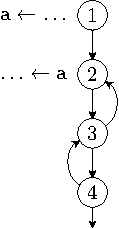
\includegraphics{liveness_dataflow_a.pdf}
       \hspace{2cm}
       \label{fig:liveness_dataflow:a}
     }
     \subfloat[Loop-nesting forest]{
       \label{fig:liveness_dataflow:b}
       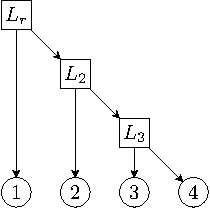
\includegraphics{liveness_dataflow_b.pdf}
     }
   \end{center}
   \caption{Bad case for iterative data-flow analysis.}
   \label{fig:liveness_dataflow}
\end{figure}


 \subsection{Liveness Sets on Irreducible Flow Graphs}
\label{sec:irreducible}

The algorithms based on loops that we described above, are only valid for reducible graphs.
We can derive an algorithm that works for irreducible graphs as well, in the following way:
transform, the irreducible graph to a reducible graph, such that the liveness in both graphs is \emph{equivalent}.
First of all we would like to stress two points:
\begin{asparaenum}[(1)]
\item
	As opposed to well-known CFG transformations such as node splitting~\cite{JC97,ASU06} our transformation does not involve any size explosion.
The key reason is that we do not impose the transformed graph to be \emph{semantically equivalent} to the original one, only isomorphism of liveness is required.
\item
	In practice the graph is not actually modified, but Algorithm~\ref{alg:dag_dfs} can be changed to simulate the modification of some edges, on the fly.
\end{asparaenum}

The transformation can be done for any \emph{minimal} loop-nesting forest as defined by Ramalingam but is simpler to explain and implement when each loop as a unique header, in particular with Havlak's loop-nesting forest.
As we will see further, the transformation, in this case, simply relies in redirecting any edge $(s,t)$ to the header of the outermost loop (if exists) that contain~$t$ but not~$s$.

For loop-nesting forests with multiple headers per loop, similarly to Ramalingam%
\footnote{Our transformation differs from the one proposed by Ramalingam as we want to keep the liveness information here, not only the dominance.}%
~\cite{ramalingam:2002:loopforest:minimal} we can add a dummy node to represent the headers.
As it allows a simple proof by induction, we give here an iterative construction that transforms each irreducible loop into a reducible one.
Performing the transformation this way, and especially from inner to outer loops would obviously lead, in the worst case, to a quadratic number of edge redirections.
As mentioned earlier, in practice edges are virtually and directly redirected to the header (or representative) of the outermost loop.

For every loop~$L$, $\textit{EntryEdges}(L)$ denotes the set of entry-edges, \ie the edges leading, from a basic block that is not part of the loop~$L$, to a block within~$L$.
$\textit{Entries}(L)$ denotes the set of~$L$'s entry-nodes, \ie the nodes that are target of an entry-edge.
Similarly, $\textit{PreEntries}(L)$ denotes the set of blocks that are the source of an entry-edge.
The set of loop-edges is given by $\textit{LoopEdges}(L)$.
Given a loop~$L$ from a graph $G = (V, E, r)$, we define the graph $\Psi_L (G) = (E', V', r)$ as follows.
The graph is extended by a new node $\delta_L$, which represents the (unique) loop-header of~$L$ after the transformation.
All edges entering the loop from preentry-nodes are redirected to this new header.
The loop-edges of~$L$ are similarly redirected to $\delta_L$ and additional edges are inserted leading from $\delta_L$ to~$L$'s former loop-headers.
More formally:
%
\begin{eqnarray*}
%  V' & = & V \cup \{\delta_L\} \\
  E' & = & E \setminus \textit{LoopEdges}(L) \setminus \textit{EntryEdges}(L)
%\\
%     &   &
\cup \{ (s, \delta_L)~|~s \in \textit{PreEntries}(L) \} \\
     &   & \cup \{ (s, \delta_L)~|~\exists (s, h) \in \textit{LoopEdges}(L) \}
%\\
%     &   &
\cup \{ (\delta_L, h)~|~h  \in \textit{LoopHeaders}(L) \}
\end{eqnarray*}
%
Repeatedly applying this transformation yields a reducible graph, slightly larger than the original graph, in which each node is still reachable from the root~$r$.
As already mentioned, depending on the order in which loops are considered, entry-edges may be updated several times during the processing in order to reach their final positions.
But the loop-nesting forest structure remains the same.
The next example illustrates this transformation.

\begin{figure}[t]
  \begin{center}
    \subfloat[Irreducible CFG~$G$] {
      \label{fig:examplecfg:a}
      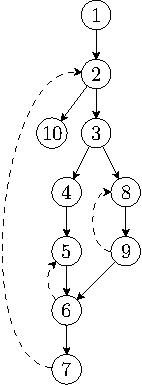
\includegraphics{examplecfg_a.pdf}
    }
    \hspace{4mm}
    \subfloat[Reducible CFG $\Psi_L(G)$; general case] {
      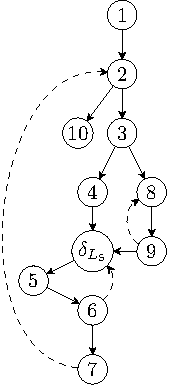
\includegraphics{examplecfg_b.pdf}
      \label{fig:examplecfg:b}
    }
    \hspace{4mm}
    \subfloat[~~Reducible CFG; single header case] {
      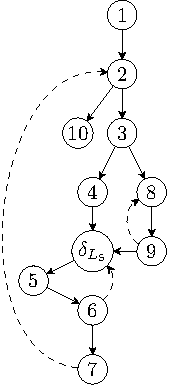
\includegraphics{examplecfg_b.pdf}
      \label{fig:examplecfg:c}
    }
  \end{center}
  \caption{%
	  A reducible CFG derived from an irreducible CFG, using the loop-nesting forest depicted in Figure~\ref{fig:exampleloop}.
	  When loops are single header, such as for Havlak's loop-nesting forests, the transformation reduces to redirect some edges.}
  \label{fig:examplecfg}
\end{figure}


\newcommand{\OLE}[2]{#1.\textsf{OLE}(#2)}

To avoid building this transformed graph explicitly, an elegant alternative is to modify the CFG traversal (Algorithm~\ref{alg:dag_dfs}).
To make things simpler, we assume that the loop-nesting forest is built so that, as in Havlak's loop-nesting forest construction, each loop~$L$ has a single loop header%
\footnote{%
	To handle loop-nesting forests with loops having several loop-headers, we can select one particular loop-header to be \emph{the} loop representative ($B_N$ in Algorithm~\ref{alg:loop_dfs}).
	But then we need to ``add'' edges from this header to the other headers of the loop.
}
, which can thus implicitly be fused with~$\delta_L$.
It is then easy to see that, after all CFG transformations, an entry-edge $(s,t)$ is redirected from~$s$ to $\OLE{t}{s}$ the outermost loop containing~$t$ and excluding~$s$, \ie of the highest ancestor of~$t$ in the loop-nesting forest that is not an ancestor of~$s$.
Thus, whenever an entry-edge $(s,t)$ is encountered during the traversal, we just have to visit $\OLE{t}{s}$ instead of~$t$, \ie to visit the representative of the largest loop containing the edge target, but not its source.
To perform this modification, we replace all occurrences of~$S$ by $\OLE{S}{B}$ at Lines~\ref{alg:dag_dfs:irreducible_dfs} and~\ref{alg:dag_dfs:irreducible} of Algorithm~\ref{alg:dag_dfs}, in order to handle irreducible flow graphs.

%% The modification follows in fact the approach used for the construction of
%% Havlak's loop-nesting forest: an edge that leads to an entry-node that is not a
%% loop-header is replaced by an edge to the loop-header. Notice that for Havlak,
%% an edge might be replaced several times, until it points to the loop-header of
%% the largest loop that does not contain its source.

\begin{example}
	Consider the CFG of Figure~\ref{fig:examplecfg:a} and the loop-nesting forest in Figure~\ref{fig:exampleloop}.
	An artificial root node~$r$ for the entire CFG have been added to turn it into a tree.
	The loop $L_5$ containing the nodes~$5$ and~$6$ is irreducible as it has two entry-nodes, via the preentry-nodes~$4$ and~$9$.
	We suppose that node~$5$ was selected as its loop-header.
	The transformed reducible graph $\Psi_{L_5}(G)$ is depicted in Figure~\ref{fig:examplecfg:b}.
	The graph might not reflect the semantics of the original program during execution, but it preserves the liveness properties of the original graph for a strict SSA program, as we will show in Theorem~\ref{thm:equiv}.
	As for Havlak's loop nesting forest, the original irreducible loop $L_5$ has a single loop-header~$5$ that can play the role of the loop-header of the transformed reducible loop (in place of $\delta_{L_5}$):
	in Figure~\ref{fig:examplecfg:c} edge $(9,6)$ is simply redirected to~$5$ the highest loop-nesting forest ancestor of~$6$ not ancestor of~$9$.
	\qed
\end{example}

\newcommand{\couple}[2]{\langle#1,#2\rangle}
\def\sep{,$ $}

\subsection{Computing the outermost excluding loop}
\label{sec:ole}
Finding the maximal loop not containing a node~$s$ but containing a node~$t$ is a problem similar to finding the least common ancestor (LCA) of the two nodes~$s$ and~$t$ in the rooted loop-nested forest:
the loop in question is the only direct child of $\textsf{LCA}(s,t)$, ancestor of~$t$.
As described in~\cite{BenderFC00} and explained in Section~\ref{sec:foundations}, an LCA query can be reduced to an RMQ query that can itself be answered in $O(1)$, with a pre-computation of $O(n)$.
Recall that the reduction to the RMQ problem is based on the Euler tour of the tree, that is the sequence of nodes as they are visited by a depth first search (DFS).
On the example of Figure~\ref{fig:exampleloop} such a tour would create the array% $A=[\couple{L_R}{0}\sep \couple{1}{1}\sep \dots\sep \couple{\textbf{2}}{2}\sep \couple{L_2}{1}\sep \couple{3}{2}\sep \couple{L_2}{1}\sep\dots\sep \couple{\textbf{9}}{3}\sep \couple{L_8}{2}\sep \couple{L_2}{1}\sep \couple{L_5}{2}\sep \couple{5}{3}\sep \couple{L_5}{2}\sep \couple{\textbf{6}}{3}\sep \dots]$ that reports between chevrons both the id of the visited node and its level, \ie its distance from $L_R$, in the tree.
Between the (unique) occurrences of the leafs~$9$ and~$6$ the occurrence of minimum level in~$A$ is $\couple{L_2}{1}$, found in $O(1)$, gives $L_2$ as the LCA of~$9$ and~$6$.
On this example, the outermost loop containing~$6$ but excluding~$9$ is $L_5$, given by the occurrence $\couple{L_5}{2}$ just following the occurrence of the \@LCA.
The attentive reader would have noticed that another order used for the Euler tour could show $\couple{L_8}{2}$ as the immediate following occurrence of $\couple{L_5}{2}$.
Also, there might exists more than one occurrence of the same node in a sub-array of~$A$:
suppose for example that we are looking for the outermost loop containing~$9$ but excluding~$2$, then $L_2$, the LCA of~$9$ and~$2$ is visited multiple times in between\ldots

To make sure that the loop-node we are looking for, \ie the outermost loop containing~$t$ and excluding~$s$, occurs in~$A$ just after the queried $\textsf{RMQ}(s,t)$, we do the following:
\begin{enumerate}
\item
	take a topological order of the forward CFG, and visit the children of each node along this order during the DFS of the Euler tour.
\item
	restrict to queries such that~$s$ is before~$t$ in the topological order used for the Euler tour.
	Notice that this condition will always be fulfilled if~$s$ dominates~$t$ or if $(s,t)$ is a forward edge of the \@CFG.
\item
	parametrize the RMQ algorithm to pick up the \emph{last} occurrence of minimum level.
\end{enumerate}

This gives a sophisticated but $\langle O(n),O(1)\rangle$ solution the OLE problem, that we will not develop further as in practice maximum loop-depth is usually small.
Simpler solutions can be used such as the naive one that would just walk upward in the tree starting at both nodes and stops when it encounters a common ancestor.

The other alternative method (shown in Algorithm~\ref{alg:hnca}) is to pre-compute the set of ancestors from the loop-tree for every node.
Then a simple set operation can find the node we are looking for:
the ancestor of the definition node are removed from the ancestor of the query point.
From the remaining ancestors, we pick the shallowest.
Using bitsets, indexed with a topological order of the loop tree, this operations are easily implemented.
The removal is a \texttt{bit-inversion} followed by a \texttt{bitwise-and} operation, and the shallowest node is found by searching for the \texttt{first-bit-set} in the bitset.
Since the number of loops (and thus the number loop-headers) is rather small, the bitsets are themselves small as well and this optimization does not result in much wasted space.

Consider a topological indexing of loop-headers accessible using:
$n.LTindex$ ($n$~being a loop-header) or reciprocally $i.node$ ($i$~being an index).
For each node, we need a bitset (indexed by loop-headers) of all its ancestors in the loop tree:
$n.ancestors$.
This can be computed using any topological traversal of the loop-tree by a call of \textsc{DFS\_compute\_ancestors}($L_r$).
Notice that some compiler intermediate representation sometimes consider $L_r$ as a loop header.
Considering so in \textsc{DFS\_compute\_ancestors} will not spoil the behavior of \@OLE.

\begin{algorithm}
  \Func{DFS\_compute\_ancestors(node~$n$)}{
    \uIf{$n \neq L_r$}{
      $n.ancestors \gets n.LTparent.ancestors$\;
    }
    \Else{
      $n.ancestors \gets bitset\_{empty}$\;
    }
    \If{$n.isLoopHeader$}{
      $n.ancestors.add(n.LTindex)$
    }
    \For{$s$ in $n.LTchildren$}{
      \textsc{DFS\_compute\_ancestors}($s$)
    }
  }
\caption{Compute the loop-nesting forest ancestors.}
\label{alg:ancestors}
\end{algorithm}

Using this information, finding the outermost excluding loop can be done by simple bitset operations:
\begin{algorithm}
  \Func{OLE(node $self$, node~$b$)}{
    $nCA \gets bitset\_and(self.ancestors, bitset\_not(b.ancestors))$\;
    \uIf{$nCA.isempty$}{
      \Return $self$
    }\Else{
      \Return $nCA.bitset\_leading\_set.node$\;
    }
  }
\caption{Outermost excluding loop.}
\label{alg:hnca}
\end{algorithm}

\begin{example}
	Consider the example of Figure~\ref{fig:exampleloop} again and suppose the loops $L_2$, $L_8$, and $L_5$ are respectively indexed~$0$,$1$, and~$2$.
	Using big-endian notations for bitsets Algorithm~\ref{alg:ancestors} would give the labels to nodes~$9$ and~$6$, $110$ and $101$ respectively.
	The outermost loop containing~$6$ but not~$9$ is given by the leading bit of $101\wedge \lnot 110=001$ \ie $L_5$.
\end{example}

\subsubsection{Correctness}
\label{sec:equiv_correctness}

We now prove that, for strict SSA programs, the liveness of the resulting reducible CFG is equivalent to the liveness of the original \@CFG.
The following results hold even for a loop-nesting forest whose loops can have more than one loop-header.
First, to be able to apply the lemmas and algorithms of Section~\ref{sec:forreducible} to the reducible CFG $\Psi_L(G)$, we need to prove that any definition of a variable still dominates its uses.

\begin{lemma}
\label{lemma:dom_psi}
If~$d$ dominates~$u$ in~$G$, then~$d$ dominates~$u$ in $\Psi_L(G)$.
\end{lemma}

It remains to show that, for every basic block present in both graphs, the live-in and live-out sets are the same.
This is proved by the following theorem.
\begin{theorem}
\label{thm:equiv}
Let $\var{v}$ be an SSA variable, $G$ a CFG, transformed into $\Psi_L(G)$ when considering a loop~$L$ of a loop-nesting forest of~$G$.
%If the definition and the uses of $\var{v}$ are
%placed in the same nodes in $\Psi_L (G)$, then
Then, for each node~$q$ of~$G$, $\var{v}$ is live-in (resp.\ live-out) at~$q$ in~$G$ iff $\var{v}$ is live-in (resp.\ live-out) at~$q$ in~$\Psi_L (G)$.
\end{theorem}




\section{Liveness Sets using Path Exploration}
\label{sec:path-explore}

Another maybe more intuitive way of calculating liveness sets is closely related to the definition of the live-range of a given variable.
As recalled earlier, a variable is live at a program point p, if p belongs to a path of the CFG leading from a definition of that variable to one of its uses without passing through the definition.
Therefore, the live-range of a variable can be computed using a backward traversal starting at its uses and stopping when reaching its (unique) definition.
This idea was first proposed by Appel in his ``Tiger'' book~\cite{appel:2002:modern} (Pages~208 and~429).
We distinguish two implementation variants of the basic idea.



\subsection{Processing Variables by Use}
\label{sec:llvm-like}

The first variant relies solely on the CFG of the input program and does not require any additional preprocessing step.
Starting from a use of a variable, all paths where that variable is live are followed by traversing the CFG backwards until the variable's definition is reached.
Along the encountered paths, the variable is added to the live-in and live-out sets of the respective basic blocks.

Algorithm~\ref{alg:use_by_use} performs the initial traversal discovering the uses of all variables in the program.
Every use is the starting point for a path exploration performed by Algorithm~\ref{alg:up_and_mark}.
The presented algorithm has also some similarities with the liveness algorithm used by the open-source compiler infrastructure \@LLVM.

 \begin{algorithm}[H]
     \Func{Compute\_LiveSets\_SSA\_ByUse(CFG)}{
       \For(\Comment Consider all blocks successively){each basic block~$B$ in CFG}{
         \For(\Comment Used in the $\phi$ of a successor block){each $v\in\PhiUses(B)$}{
           $\LiveOut(B)= \LiveOut(B)\union\{v\}$\;
           \textsf{Up\_and\_Mark}($B,v$)\;
         }
         \For(\Comment Traverse~$B$ to find all uses){each~$v$ used in~$B$ ($\phi$ excluded)}{
         \textsf{Up\_and\_Mark}($B,v$)\;
         }
       }
     }
   \caption{Compute liveness sets by exploring paths from variable uses.}
   \label{alg:use_by_use}
 \end{algorithm}

\begin{algorithm}[H]
  \Func{Up\_and\_Mark($B,v$)}{
    \If{$\Def(v) \in B$ ($\phi$ excluded)}{
      return \Comment{Killed in the block, stop}
    }
    \If{$v\in \LiveIn(B)$}{
      return \Comment{Propagation already done, stop}
    }
    $\LiveIn(B)= \LiveIn(B) \union \{v\}$\;
    \If{$v\in\PhiKill(B)$}{
      return \Comment{Do not propagate $\phi$ definitions}
    }
    \For(\Comment Propagate backward){each $P\in\textrm{CFG\_preds}(B)$}{
      $\LiveOut(P)=\LiveOut(P)\union\{v\}$\;
      \textsf{Up\_and\_Mark}($P,v$)\;
    }
  }
  \caption{Explore all paths from a variable's use to its definition.}
  \label{alg:up_and_mark}
\end{algorithm}

\subsection{Processing Variables by Definition}
\label{sec:Appel-like}

The second variant follows the initial idea of Appel~\cite[p.~429]{appel:2002:modern}, but adapted and optimized to work on blocks instead of instructions.
Depending on the particular compiler framework, a preprocessing step that performs a full traversal of the program (\ie the instructions) might be required in order to derive the def-use chains for all variables, \ie a list of all uses for each SSA-variable.
% In contrast to the previous use-by-use variant, it is not necessary to explicitly scan the program for uses of each variable when def-use chains are available.
Algorithm~\ref{alg:var_by_var} adapts the pseudo-code shown previously to make use of these def-use chains.
The algorithm to perform the path exploration stays the same, \ie Algorithm~\ref{alg:up_and_mark}.

\begin{algorithm}[H]
    \Func{Compute\_LiveSets\_SSA\_ByVar(CFG)}{
      \For{each variable~$v$}{
        \For{each block~$B$ where~$v$ is used}{
            \If(\Comment Used in the $\phi$ of a successor block){$v \in \PhiUses(B)$}{
              $\LiveOut(B)=\LiveOut(B)\union\{v\}$\;
            }
            \textsf{Up\_and\_Mark}($B,v$)\;
        }
      }
    }
  \caption{Compute liveness sets per variable using def-use chains.}
  \label{alg:var_by_var}
\end{algorithm}

A nice property of this approach is that the processing of different variables is not intermixed, \ie the processing of one variable is completed before the processing of another variable begins.
This enables to optimize the \textsf{Up\_and\_Mark} phase by using a stack-like set representation.
Unlike in Algorithm~\ref{alg:up_and_mark}, the expensive set-insertion operations and set-membership tests can then be avoided.
It is indeed sufficient to test the top element of the stack, see Algorithm~\ref{alg:up_and_mark_stack}.
Note also that, in strict SSA, in a given block, no use can appear before a definition.
Thus, if $\var{v}$ is live-out or used in a block~$B$, it is live-in iff it is not defined in~$B$.

\begin{algorithm}[H]
    \Func{Up\_and\_Mark\_Stack($B,v$)}{
      \If{$\Def(v)\in B$ ($\phi$ excluded)}{
        return \Comment {Killed in the block, stop}
      }
      \If{$\top(\LiveIn(B)) = v$}{
        return \Comment {propagation already done, stop}
      }
      $\push(\LiveIn(B), v)$\;
     \If{$v\in\PhiKill(B)$}{
       return \Comment {Do not propagate $\phi$ definitions}
     }
     \For(\Comment Propagate backward){each $P\in\textrm{CFG\_preds}(B)$}{
       \If{$\top(\LiveOut(P)) \neq v$}{
         $\push(\LiveOut(P),v)$
       }
       \textsf{Up\_and\_Mark\_Stack}($P,v$)\;
      }
    }
  \caption{Optimized path exploration using a stack-like data structure.}
  \label{alg:up_and_mark_stack}
\end{algorithm}

\subsection{Path Exploration for non-SSA-form Programs}
\label{sec:path-explore:non_ssa}

Interestingly, we can show that, with an additional preprocessing step, the path exploration approach can also be applied to programs that are \emph{not} in SSA form.
Similar to the precomputation of the def-use chains for the variable-by-variable approach (Section~\ref{sec:Appel-like}), we can avoid multiple traversals of the internal program representation by precomputing information on uses and definitions of all variables in the program.
First, using a forward scan of each block (see Algorithm~\ref{alg:precomputeusesdefs}), we compute, for each variable~$v$, the list of blocks, denoted by \UpExp($v$), where~$v$ is live-in and upward-exposed, \ie the blocks where the first access to~$v$ is a use and not a definition.
We also compute the list of blocks, denoted by \Kill($v$), where the variable is defined.

\begin{algorithm}[H]
  \Func{Compute\_Killing\_and\_UpwardExposed\_Stack(CFG)}{
    \For{each basic block~$B$ in the CFG}{
      \For{each access to a variable~$v$, from start to end of block}{
        \If(\Comment No definition yet){$\top(\Kill(v)) \neq B$}{
          \If(\Comment Upward-exposed use at~$B$){$v$ is a use}{
            \uIf{$\top(\UpExp(v)) \neq B$}{
              $\push(\UpExp(v), B)$\;
            }
            \Else{
              $\push(\Kill(v), B)$ \Comment First definition in~$B$
            }
          }
        }
      }
    }
  }
  \caption{Compute the upward-exposed uses and definitions of variables.}
  \label{alg:precomputeusesdefs}
\end{algorithm}

The algorithm to compute the liveness information is similar to the optimized variable-by-variable algorithm presented in the previous section.
The main difference is that multiple definitions of the same variable might appear in the program.
In order to avoid expensive checks to find definitions during the path exploration, basic blocks are marked with a variable during the processing.
The marking indicates that the path exploration algorithm should stop following the current path any further.
Also, when the variable is already known to be live-in, the path exploration stops.
% A block is marked with the current variable in two cases:
%\begin{compactenum}[(1)]
%\item
%	The basic block contains a definition of the variable or
%\item
%	The basic block has been visited by the path exploration algorithm previously, the variable is thus already known to be live.
%\end{compactenum}
Algorithms~\ref{alg:var_by_var_non_ssa} and~\ref{alg:up_and_mark_non_ssa} show the modified pseudo-code of the liveness algorithm for programs that are not in SSA form.

\begin{algorithm}[H]
    \Func{Compute\_LiveSets\_NonSSA\_ByVar\_Stack(CFG)}{
       \For{each basic block~$B$ of CFG}{
         mark~$B$ with $\vundef$
       }
      \For{each variable~$v$}{
        \For{each block~$B$ in $\Kill(v)$}{
          mark~$B$ with~$v$
        }
        \For{each block~$B$ in $\UpExp(v)$}{
          \If(\Comment Not propagated yet){$\top(\LiveIn(B)) \neq v$}{
            $\push(\LiveIn(B),v)$ \Comment Insert in live-in set\\
            \For(\Comment Propagate backward){$P\in\textrm{CFG\_preds}(B)$}{
              \textsf{Up\_and\_Mark\_NonSSA\_Stack}($P,v$)\;
            }
          }
        }
      }
    }
  \caption{Compute liveness per variable for non-SSA-form programs.}
  \label{alg:var_by_var_non_ssa}
\end{algorithm}

\begin{algorithm}[H]
    \Func{Up\_and\_Mark\_NonSSA\_Stack($B,v$)}{
      \lIf{$\top(\LiveOut(P)) \neq v$}{$\push(\LiveOut(P),v)$}\;
      \lIf(\Comment Killed in the block, stop){$B$ is marked with~$v$}{return}
      \lIf(\Comment Already processed){$\top(\LiveIn(B)) = v$}{return}
      $\push(\LiveIn(B),v)$; \Comment Not propagated yet\\
      \For(\Comment Propagate backward){each $P\in\textrm{CFG\_preds}(B)$}{
        \textsf{Up\_and\_NonSSA\_Mark\_Stack}($P,v$)\;
      }
    }
  \caption{Compute liveness sets per variable for non-SSA-form programs.}
  \label{alg:up_and_mark_non_ssa}
\end{algorithm}


\section{Liveness Check using Loop Nesting Forest and \Reduced\ Reachability}
\label{sec:live-check}


The goal of this section is to revisit the liveness check algorithm proposed in~\cite{BoissinotHGDR08} in the light of the properties and techniques developed in sections~\ref{sec:forreducible}, \ref{sec:irreducible}, and~\ref{sec:ole} that we will recall below.

In contrast to liveness sets, liveness check does not provide the set of variables live at a block, but provides a query system to answer questions such as ``is variable $v$ live at location $q$?''.
Such a framework is well suited for tree-scan based register allocation~\cite{ColombetBBHR11}, SSA destruction~\cite{boissinot:2009:ssadestruction}, or Hyperblock scheduling.
Most register-pressure aware algorithms such as code-motion are not designed to take advantage of liveness check query system and still require sets.
On the other hand, such a query system can obviously be built on top of precomputed liveness sets.
Queries in $O(1)$ are possible, at least for basic block boundaries, providing the use of sparsesets~\cite{cooper:2004:engineering} or bitsets to allow for efficient element-wise queries.
If sets are only stored at basic block boundaries, to allow a query system at instructions granularity, the list of variables' uses or backward scans can be used.
Constant time worst case complexity is lost in this scenario and liveness sets that have to be incrementally updated at each (even minor) code transformation, can be avoided and replaced by less memory consuming data structures that only depend on the \@CFG.

For completeness, we recall the prerequisites of the liveness check query system here:
\begin{itemize}
\item
	The CFG of the input program is available.
\item
	The dominance tree of the CFG is available.
	Otherwise it is computable in $O(|V|)$.
	Within each basic block checking if one instruction precedes another should be possible in $O(1)$.
\item
	A loop-nesting forest of the CFG is available.
	Also computable in~$O(|V| \log^*|E|)$.
\item
	A list of uses for each variable, also known as def-use chain is available.
	Having an easy-to-maintain def-use chain is one of the major advantages of the SSA form.
	Hence, def-use chains are often available in SSA-based compilers.
	Updating the def-use chain when adding or removing uses of a variable incurs virtually no costs, quite contrary to updating liveness information on each change.
\end{itemize}

In the following, we consider the live-in query of variable $\var{a}$ at node $q$.
To avoid notational overhead, let $\var{a}$ be defined in the CFG node $d:=\ldef{a}$ and let $u \in \luse{a}$ be (w.l.o.g.) the single node where $\var{a}$ is used.
Suppose that $q$ is strictly dominated by $d$ (otherwise $v$ cannot be live at $q$).
Lemmas~\ref{lemma:firstpass}, \ref{lemma:firstpass2}, and~\ref{lemma:secondpass} stated in Section~\ref{sec:equiv_correctness} can be simplified as follow:
\begin{enumerate}
\item
	Let $h$ be the header of the maximal loop containing $q$ but not $d$.
	Let $h$ be $q$ if such maximal loop does not exist.
	Then $v$ is live-in at $h$ if and only if there exists a forward path that goes from $h$ to $u$.
\item
	If $v$ is live-in at the header of a loop then it is live at any node inside the loop.
\end{enumerate}

In other words, $v$ is live-in at $q$ if and only if there exists a forward path from $h$ to $u$ where $h$ is, if exists, the header of the maximal loop containing $q$ but not $d$, $q$ itself otherwise.
Given the \reducedGraph\ and the loop nesting forest, finding out if a variable is live at some program point can be done in two steps.
First, if there exists a loop containing the program point $q$ and not the definition, pick the header of the biggest such loop instead as the query point.
Then check for reachability from $q$ to any use of the variable in the forward \@CFG.
As explained in Section~\ref{sec:irreducible}, for irreducible CFG, the modified forward control-flow graph that redirects any edge $(s,t)$ to the loop header of the outermost loop containing $t$ but excluding $s$ ($\OLE{t}{s}$), has to be used instead.
Correctness is proved from the theorems used for liveness sets.

\newcommand{\BB}[1]{\textsf{basicBlock}(#1)}
\newcommand{\ordering}[1]{\textsf{order}(#1)}
\newcommand{\isLoopHeader}[1]{\textsf{isLoopHeader}(#1)}
\newcommand{\FR}[2]{\textsf{{\reduced}Reachable}(#1,#2)}

Algorithm~\ref{alg:liveinchk} puts a little bit more efforts onto the table to provide a query system at instructions granularity.
If $q$ is in the same basic block than $d$ (lines~6-10, then $v$ is live at $q$ if and only if there is a use outside the basic block, or inside but after $q$.
If $h$ is a loop-header then $v$ is live at $q$ if and only if a use is forward reachable from $h$ (lines~17-18).
Otherwise, if the use is in the same basic block than $q$ it must be after $q$ to bring the variable live at $q$ (lines 15-16).
In this pseudo-code, upper cases are used for basic blocks while lower case are used for program points at instructions granularity.
\texttt{def(a)} is an operand.
\texttt{uses(a)} is a set of operands.
\texttt{\BB{u}} returns the basic block containing the operand \texttt{u}.
Given the semantics of the \phifun instruction, the basic block returned by this function for a \phifun operand can be different from the block where the instruction textually occurs.
Also, \texttt{u.order} provides the corresponding (increasing) ordering in the basic block.
For a \phifun\ operand, the ordering number might be greater than the maximum ordering of the basic block if the semantics of the \phifun\ places the uses on outgoing edges of the predecessor block.
\OLE{Q}{D}\ corresponds to Algorithm~\ref{alg:hnca} given in Section~\ref{sec:ole}.
\FR{H}{U}\ that tells if $U$ is reachable in the modified forward CFG will be described further.

\begin{algorithm}
  \Func{IsLiveIn(programPoint $q$, var $\var{a}$)}{
    $d \gets \ldef{a}$\;
    $D \gets \BB{d}$; $Q \gets \BB{q}$\;
    \If{$\textsf{not} \left(\strut D \sdom Q \textsf{ or } (D = Q \textsf{ and } \ordering{d} < \ordering{q})\right)$}{
      \Return $\textit{false}$\;
    }
    \If{$Q = D$}{
      \For{$u \textbf{ in } \luse{\var{a}}$}{
        $U\gets \BB{u}$\;
        \If{$U \neq D \textsf{ or } \ordering{q} \leq \ordering{u}$}{
	  \Return $\textit{true}$\;
        }
      }
      \Return $\textit{false}$\;
    }
    $H \gets \OLE{Q}{D}$\;
    \For{$u \textbf{ in } \luse{\var{a}}$}{
      $U\gets \BB{u}$\;
      \If{$\left(\textsf{not }\isLoopHeader{H}\right) \textsf{ and } U = Q  \textsf{ and } \ordering{u} < \ordering{q}$}{
        $\textbf{continue}$\;
      }
      \If{$\FR{H}{U}$}{
        \Return $\textit{true}$\;
      }
    }
    \Return $\textit{false}$\;
  }
\caption{Live-In Check.}
\label{alg:liveinchk}
\end{algorithm}

Live-out check algorithm given by Algorithm~\ref{alg:liveoutchk} only differs from Live-in check in lines~4, 9, and~14 that involve ordering comparisons.
In line~4, if $q$ is equal to $d$ it cannot be live-in while it might be live-out; in lines~9 and~15 if $q$ is at a use point it makes it live-in but not necessarily live-out.

\begin{algorithm}
  \Func{IsLiveOut(programPoint $q$, var $\var{a}$)}{
     $d \gets \ldef{\var{a}}$\;
     $D \gets \BB{d}$; $Q \gets \BB{q}$\;
    \If(\Comment{q must be dominated by the definition}){$\textsf{not} \left(\strut D \sdom Q \textsf{ or } (D = Q \textsf{ and } \ordering{d} \leq \ordering{q})\right)$}{
       \Return $\textit{false}$\;
    }
    \If{$Q = D$}{
      \For{$u \textbf{ in } \luse{\var{a}}$}{
         $U\gets \BB{u}$\;
	\If{$U \neq D \textsf{ or } \ordering{q} < \ordering{u}$}{
	   \Return $\textit{true}$\;
	}
      }
       \Return $\textit{false}$\;
    }
     $H \gets \OLE{Q}{D}$\;
    \For{$u \textbf{ in } \luse{\var{a}}$}{
       $U\gets \BB{u}$\;
      \If{$\left(\textsf{not } \isLoopHeader{H}\right) \textsf{ and } U = Q  \textsf{ and } \ordering{u} \leq \ordering{q}$}{
	 $\textbf{continue}$\;
      }
      \If{$\FR{H}{U}$}{
	\Return $\textit{true}$
      }
    }
     \Return $\textit{false}$\;
  }
  \caption{Live-Out Check.}
  \label{alg:liveoutchk}
\end{algorithm}


\subsection{Computing the modified-\reduced\ reachability}

The liveness check query system relies on pre-computations for efficient \textsf{OLE} and \textsf{{\reduced}Reachable} queries.
The outermost excluding loop is identical to the one used for liveness set.
We explain how we compute the modified-\reduced\ reachability here.
In practice we do not build explicitly the modified-\reduced\ graph.
To compute efficiently the modified-\reduced\ reachability we simply need to traverse the modified-\reduced\ graph in a reverse topological order.
A post-order initiated by a call to the recursive function \textsf{DFS\_Compute\_{\reduced}Reachable}($r$) (Algorithm~\ref{alg:computeFR}) will do the job.
Bitsets can be used to efficiently implement sets of basic blocks.
Once forward reachability have been pre-computed this way, $\FR{H}{U}$ returns true if and only if $U\in H.{\reduced}Reachable$.

\begin{algorithm}
  \Func{DFS\_Compute\_{\reduced}Reachable(block $N$)}{
     $N.\textsf{{\reduced}Reachable} \gets \emptyset$\;
     $N.\textsf{{\reduced}Reachable.add}(N)$\;
    \For{\textbf{each} $S\in \textsf{succs}(N)$ \textbf{if} $(N,S)$ is not a loop-edge}{
       $H \gets \OLE{S}{N}$\;
       \If{$H.\textsf{{\reduced}Reachable} = \bot$}{\textsf{DFS\_Compute\_{\reduced}Reachable}$(H)$}
       $N.\textsf{{\reduced}Reachable} \gets  N.\textsf{{\reduced}Reachable} \cup H.\textsf{{\reduced}Reachable}$\;
    }
  }
\caption{Computation of modified-forward reachability using a traversal along a reverse topological order.}
\label{alg:computeFR}
\end{algorithm}



\section{Further readings}
\label{sec:liveness:further}
Liveness information is usually computed with iterative
data-flow analysis, which goes back to Kildall~\cite{K73}. The algorithms are,
however, not specialized to the computation of liveness sets and may
incur overhead. Several strategies are possible, leading to
different worst-case complexities and performance in practice. Round-robin algorithms
propagate information according to a fixed block ordering derived from a
depth-first spanning tree and iterate until it stabilizes.  The complexity of
this scheme was analyzed by Kam et al.~\cite{KU76}, see
Section~\ref{sec:data-flow}.  
Node Listing algorithms specifies, a priori, the overall sequence of nodes, where repetitions are allowed, along which data-flow equations are applied. Kennedy~\cite{Kennedy75} devises for structured flow graphs node listings of size $2|V|$, with $|v|$ the number of control-flow-nodes, and mentions the existence of node listings of size $O|V| \log(|V|)$ for reducible flow graphs.
Worklist algorithms focus on blocks that may need
to be updated because the liveness sets of their successors (for
backward problems) changed.
Empirical results by Cooper et al.~\cite{CHK06} indicate that the order in
which basic blocks are processed is critical and directly impacts the number of
iterations. They showed that, in practice, a mixed solution, called ``single
stack worklist'', based on a worklist initialized with a round-robin order, is
the most efficient one  for liveness analysis. In contrast, our
non-iterative data-flow algorithm requires at most two passes over the basic
blocks, in all cases. In practice, for strict SSA programs, it is on
average twice as fast as the ``single stack worklist'' approach (see
Section~\ref{sec:experiments}).

Alternative ways to solve data-flow problems belong to the family of elimination-based algorithms~\cite{RyderP86}. Through recursive reductions of the 
CFG, variables of the data-flow system are successively eliminated and equations are reduced until the CFG reduces to a single node. 
The best, but unpractical, worst case complexity elimination algorithm has an almost-linear complexity $O(|E|\alpha(|E|))$. 
It requires the CFG (resp. the reverse CFG) to be reducible for a forward (resp.  backward) analysis.
For non-reducible flow-graphs, non of the existing approaches can guarantee a worst case complexity better than $O(|E|^3)$.
In practice, irreducible CFGs are rare, but liveness
analysis is a backward data-flow problem, which frequently leads to
irreducible reverse CFGs. In contrast, the handling of irreducibility by our algorithm is extremely simple and does not change its overall linear complexity (see Section~\ref{sec:irreducible}).

Gerlek et al.~\cite{gerlek94reference} use so-called $\lambda$-operators to collect upward exposed uses at control-flow split points.
Precisely, the $\lambda$-operators are placed at the iterated dominance frontiers, computed on the reverse CFG, of the set of uses of a variable.
These $\lambda$-operators and the other uses of variables are chained together and liveness is efficiently computed on this graph representation.
The technique of Gerlek et al.~can be considered as a precursor of the live variable analysis based on the Static Single Information (SSI) form conjectured by Singer~\cite{singer:2006:phd} and revisited by Boissinot et al.~\cite{BoissinotBDR12}.
In both cases, insertion of pseudo-instructions guarantee that any definition is post-dominated by a use.

Another approach to compute liveness was proposed by
Appel~\cite[p.~429]{appel:2002:modern}. Instead of computing the liveness
information for all variables at the same time, variables are handled
individually by exploring paths in the CFG starting from variable uses. 
Using logic programming, McAllester~\cite{M02} presented an equivalent approach to show that liveness analysis can be performed in time
proportional to the number of instructions and variables.
However, his theoretical analysis is limited to a restricted input language
with simple conditional branches and instructions.
A more generalized analysis will be given later, both in terms of theoretical complexity (Section~\ref{sec:path-explore:complexity}) and of practical evaluation (Section~\ref{sec:experiments})
.For comparison, we designed optimized implementations of this path-exploration principle (see Section~\ref{sec:path-explore}), for both SSA and non-SSA programs, and compared the efficiency of the resulting algorithms with our novel non-iterative data-flow algorithm.



Liveness analysis for strict SSA was first addressed by Boissinot et
al.~\cite{BoissinotHGDR08} who introduced the liveness check approach.
Each query relies in \reduced\ reachability checks from some nodes of the CFG.
The framework developed in this paper for computing liveness sets follows the same idea of ``path decomposition'', but the use of loop-nesting forest allows to reformulate it in a more elegant and simpler way.
Wimmer et al.~\cite{WimmerF10} gave an algorithm, specialized to linear scan
register allocation, to build the ``intervals'' of basic blocks where each
variable is live. Although a possible extension to irreducible CFGs is
sketched, the algorithm restricts itself to reducible CFGs or to a form of SSA
where live-ranges are cut at loop-entry blocks with $\phi$-functions.  The algorithm
we propose is a generalization~\footnote{Actually, we designed this algorithm
  in 2009-2010 independently of~\cite{WimmerF10} (see~\cite{Boissinot10}).} for computing liveness sets: ~\cite{BoissinotHGDR08}
it uses the concept of loop-nesting forest and is proved correct with no
restriction on the~CFG, on the strict SSA form, or on the loop-nesting forest
as long as it respects the minimal properties stated by
Ramalingam~\cite{ramalingam:2002:loopforest:minimal}. As a by-product, this
proves the correctness of the algorithm of~\cite{WimmerF10} and how a suitable
order of basic blocks can be chosen thanks to a loop-nesting forest. Such
orders were also exploited for liveness analysis in static single information
(SSI)~\cite{BoissinotBDR12}.  
